% Created by tikzDevice version 0.6.1 on 2016-06-13 09:09:03
% !TEX encoding = UTF-8 Unicode
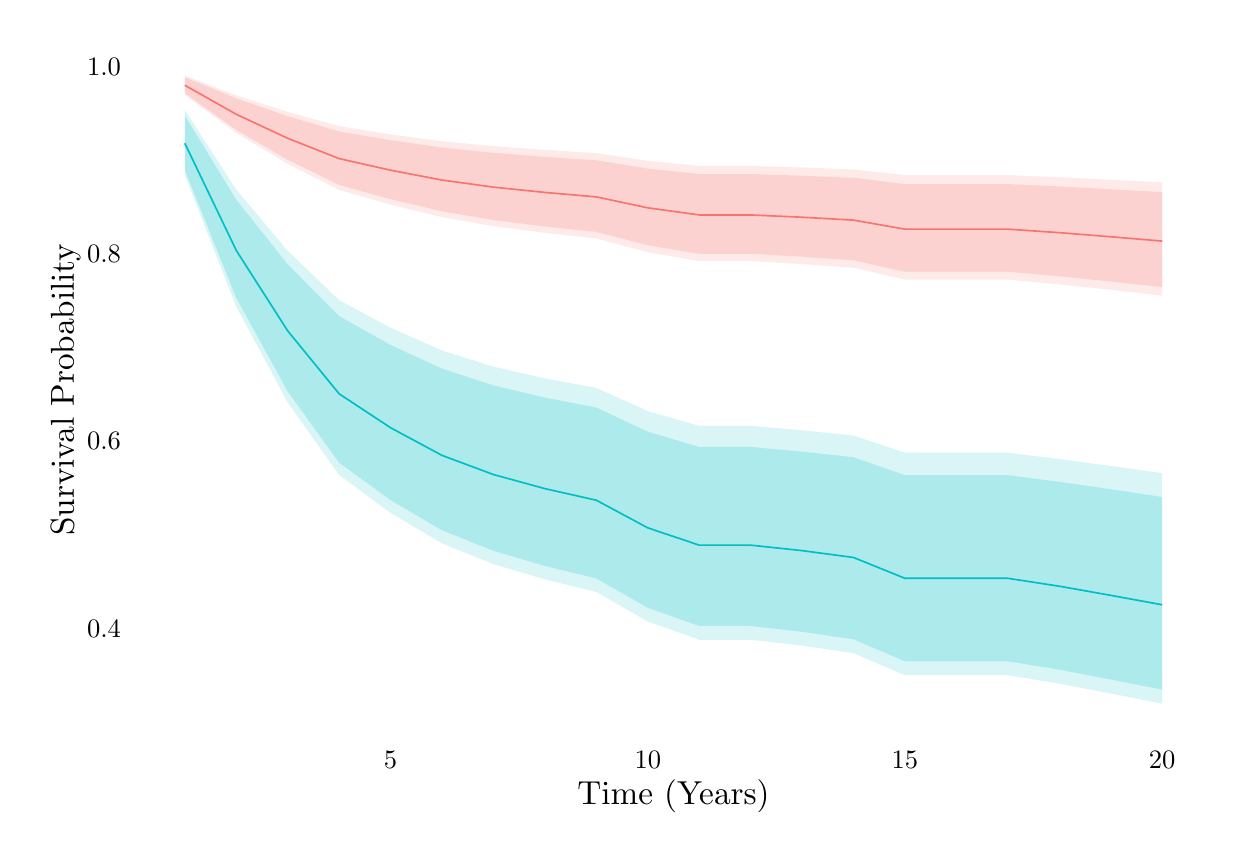
\begin{tikzpicture}[x=1pt,y=1pt]
\definecolor[named]{drawColor}{rgb}{0.00,0.00,0.00}
\definecolor[named]{fillColor}{rgb}{1.00,1.00,1.00}
\fill[color=fillColor,] (0,0) rectangle (433.62,289.08);
\begin{scope}
\path[clip] (  0.00,  0.00) rectangle (433.62,289.08);
\end{scope}
\begin{scope}
\path[clip] (  0.00,  0.00) rectangle (433.62,289.08);
\end{scope}
\begin{scope}
\path[clip] (  0.00,  0.00) rectangle (433.62,289.08);
\end{scope}
\begin{scope}
\path[clip] (  0.00,  0.00) rectangle (433.62,289.08);
\end{scope}
\begin{scope}
\path[clip] (  0.00,  0.00) rectangle (433.62,289.08);
\end{scope}
\begin{scope}
\path[clip] (  0.00,  0.00) rectangle (433.62,289.08);
\end{scope}
\begin{scope}
\path[clip] (  0.00,  0.00) rectangle (433.62,289.08);
\end{scope}
\begin{scope}
\path[clip] (  0.00,  0.00) rectangle (433.62,289.08);
\end{scope}
\begin{scope}
\path[clip] (  0.00,  0.00) rectangle (433.62,289.08);
\end{scope}
\begin{scope}
\path[clip] (  0.00,  0.00) rectangle (433.62,289.08);
\definecolor[named]{drawColor}{rgb}{1.00,1.00,1.00}
\definecolor[named]{fillColor}{rgb}{1.00,1.00,1.00}

\draw[color=drawColor,line width= 0.6pt,line cap=round,line join=round,fill=fillColor,] (  0.00,  0.00) rectangle (433.62,289.08);
\end{scope}
\begin{scope}
\path[clip] (  0.00,  0.00) rectangle (433.62,289.08);
\end{scope}
\begin{scope}
\path[clip] (  0.00,  0.00) rectangle (433.62,289.08);
\end{scope}
\begin{scope}
\path[clip] (  0.00,  0.00) rectangle (433.62,289.08);
\end{scope}
\begin{scope}
\path[clip] ( 39.13, 33.48) rectangle (427.62,283.08);
\definecolor[named]{fillColor}{rgb}{1.00,1.00,1.00}

\draw[fill=fillColor,draw opacity=0.00,] ( 39.13, 33.48) rectangle (427.62,283.08);
\definecolor[named]{drawColor}{rgb}{0.97,0.46,0.43}
\definecolor[named]{fillColor}{rgb}{0.97,0.46,0.43}

\draw[color=drawColor,line width= 0.6pt,line join=round,] ( 56.79,268.27) --
	( 75.38,257.77) --
	( 93.96,249.11) --
	(112.55,241.77) --
	(131.14,237.57) --
	(149.73,234.01) --
	(168.32,231.46) --
	(186.90,229.54) --
	(205.49,227.93) --
	(224.08,223.97) --
	(242.67,221.41) --
	(261.26,221.41) --
	(279.84,220.58) --
	(298.43,219.53) --
	(317.02,216.27) --
	(335.61,216.27) --
	(354.20,216.27) --
	(372.79,215.01) --
	(391.37,213.52) --
	(409.96,211.96);
\definecolor[named]{drawColor}{rgb}{0.00,0.75,0.77}
\definecolor[named]{fillColor}{rgb}{0.00,0.75,0.77}

\draw[color=drawColor,line width= 0.6pt,line join=round,] ( 56.79,247.29) --
	( 75.38,208.58) --
	( 93.96,179.52) --
	(112.55,156.77) --
	(131.14,144.51) --
	(149.73,134.52) --
	(168.32,127.60) --
	(186.90,122.51) --
	(205.49,118.32) --
	(224.08,108.33) --
	(242.67,102.09) --
	(261.26,102.09) --
	(279.84,100.11) --
	(298.43, 97.63) --
	(317.02, 90.10) --
	(335.61, 90.10) --
	(354.20, 90.10) --
	(372.79, 87.25) --
	(391.37, 83.95) --
	(409.96, 80.54);
\definecolor[named]{fillColor}{rgb}{0.97,0.46,0.43}

\draw[fill=fillColor,fill opacity=0.15,draw opacity=0.00,] ( 56.79,271.73) --
	( 75.38,264.63) --
	( 93.96,258.64) --
	(112.55,253.47) --
	(131.14,250.53) --
	(149.73,248.03) --
	(168.32,246.26) --
	(186.90,244.89) --
	(205.49,243.75) --
	(224.08,240.94) --
	(242.67,239.12) --
	(261.26,239.12) --
	(279.84,238.55) --
	(298.43,237.85) --
	(317.02,235.79) --
	(335.61,235.79) --
	(354.20,235.79) --
	(372.79,235.02) --
	(391.37,234.11) --
	(409.96,233.15) --
	(409.96,192.27) --
	(391.37,194.36) --
	(372.79,196.34) --
	(354.20,198.03) --
	(335.61,198.03) --
	(317.02,198.03) --
	(298.43,202.33) --
	(279.84,203.68) --
	(261.26,204.74) --
	(242.67,204.74) --
	(224.08,207.95) --
	(205.49,212.92) --
	(186.90,214.95) --
	(168.32,217.37) --
	(149.73,220.62) --
	(131.14,225.14) --
	(112.55,230.50) --
	( 93.96,239.87) --
	( 75.38,251.05) --
	( 56.79,264.84) --
	cycle;
\definecolor[named]{fillColor}{rgb}{0.00,0.75,0.77}

\draw[fill=fillColor,fill opacity=0.15,draw opacity=0.00,] ( 56.79,259.26) --
	( 75.38,230.54) --
	( 93.96,208.42) --
	(112.55,190.63) --
	(131.14,180.62) --
	(149.73,172.42) --
	(168.32,166.56) --
	(186.90,162.34) --
	(205.49,158.89) --
	(224.08,150.48) --
	(242.67,145.20) --
	(261.26,145.20) --
	(279.84,143.59) --
	(298.43,141.67) --
	(317.02,135.48) --
	(335.61,135.48) --
	(354.20,135.48) --
	(372.79,133.20) --
	(391.37,130.70) --
	(409.96,128.06) --
	(409.96, 44.82) --
	(391.37, 48.47) --
	(372.79, 52.05) --
	(354.20, 55.08) --
	(335.61, 55.08) --
	(317.02, 55.08) --
	(298.43, 63.06) --
	(279.84, 65.78) --
	(261.26, 67.90) --
	(242.67, 67.90) --
	(224.08, 74.50) --
	(205.49, 85.17) --
	(186.90, 89.71) --
	(168.32, 95.24) --
	(149.73,102.72) --
	(131.14,113.74) --
	(112.55,127.43) --
	( 93.96,153.70) --
	( 75.38,188.26) --
	( 56.79,235.76) --
	cycle;
\definecolor[named]{fillColor}{rgb}{0.97,0.46,0.43}

\draw[fill=fillColor,fill opacity=0.20,draw opacity=0.00,] ( 56.79,271.18) --
	( 75.38,263.52) --
	( 93.96,257.09) --
	(112.55,251.56) --
	(131.14,248.41) --
	(149.73,245.73) --
	(168.32,243.83) --
	(186.90,242.37) --
	(205.49,241.15) --
	(224.08,238.15) --
	(242.67,236.20) --
	(261.26,236.20) --
	(279.84,235.59) --
	(298.43,234.83) --
	(317.02,232.57) --
	(335.61,232.57) --
	(354.20,232.57) --
	(372.79,231.71) --
	(391.37,230.70) --
	(409.96,229.64) --
	(409.96,195.34) --
	(391.37,197.35) --
	(372.79,199.25) --
	(354.20,200.88) --
	(335.61,200.88) --
	(317.02,200.88) --
	(298.43,205.02) --
	(279.84,206.33) --
	(261.26,207.35) --
	(242.67,207.35) --
	(224.08,210.46) --
	(205.49,215.28) --
	(186.90,217.24) --
	(168.32,219.58) --
	(149.73,222.73) --
	(131.14,227.10) --
	(112.55,232.28) --
	( 93.96,241.34) --
	( 75.38,252.12) --
	( 56.79,265.39) --
	cycle;
\definecolor[named]{fillColor}{rgb}{0.00,0.75,0.77}

\draw[fill=fillColor,fill opacity=0.20,draw opacity=0.00,] ( 56.79,257.31) --
	( 75.38,226.89) --
	( 93.96,203.55) --
	(112.55,184.86) --
	(131.14,174.41) --
	(149.73,165.87) --
	(168.32,159.80) --
	(186.90,155.40) --
	(205.49,151.80) --
	(224.08,143.07) --
	(242.67,137.58) --
	(261.26,137.58) --
	(279.84,135.89) --
	(298.43,133.85) --
	(317.02,127.37) --
	(335.61,127.37) --
	(354.20,127.37) --
	(372.79,124.96) --
	(391.37,122.29) --
	(409.96,119.48) --
	(409.96, 49.90) --
	(391.37, 53.54) --
	(372.79, 57.09) --
	(354.20, 60.12) --
	(335.61, 60.12) --
	(317.02, 60.12) --
	(298.43, 68.07) --
	(279.84, 70.77) --
	(261.26, 72.88) --
	(242.67, 72.88) --
	(224.08, 79.45) --
	(205.49, 90.06) --
	(186.90, 94.56) --
	(168.32,100.05) --
	(149.73,107.46) --
	(131.14,118.36) --
	(112.55,131.87) --
	( 93.96,157.65) --
	( 75.38,191.42) --
	( 56.79,237.59) --
	cycle;
\end{scope}
\begin{scope}
\path[clip] (  0.00,  0.00) rectangle (433.62,289.08);
\end{scope}
\begin{scope}
\path[clip] (  0.00,  0.00) rectangle (433.62,289.08);
\end{scope}
\begin{scope}
\path[clip] (  0.00,  0.00) rectangle (433.62,289.08);
\end{scope}
\begin{scope}
\path[clip] (  0.00,  0.00) rectangle (433.62,289.08);
\end{scope}
\begin{scope}
\path[clip] (  0.00,  0.00) rectangle (433.62,289.08);
\end{scope}
\begin{scope}
\path[clip] (  0.00,  0.00) rectangle (433.62,289.08);
\definecolor[named]{drawColor}{rgb}{0.00,0.00,0.00}

\node[color=drawColor,anchor=base east,inner sep=0pt, outer sep=0pt, scale=  0.96] at ( 33.73, 68.88) {0.4%
};

\node[color=drawColor,anchor=base east,inner sep=0pt, outer sep=0pt, scale=  0.96] at ( 33.73,136.57) {0.6%
};

\node[color=drawColor,anchor=base east,inner sep=0pt, outer sep=0pt, scale=  0.96] at ( 33.73,204.26) {0.8%
};

\node[color=drawColor,anchor=base east,inner sep=0pt, outer sep=0pt, scale=  0.96] at ( 33.73,271.95) {1.0%
};
\end{scope}
\begin{scope}
\path[clip] (  0.00,  0.00) rectangle (433.62,289.08);
\end{scope}
\begin{scope}
\path[clip] (  0.00,  0.00) rectangle (433.62,289.08);
\end{scope}
\begin{scope}
\path[clip] (  0.00,  0.00) rectangle (433.62,289.08);
\end{scope}
\begin{scope}
\path[clip] (  0.00,  0.00) rectangle (433.62,289.08);
\end{scope}
\begin{scope}
\path[clip] (  0.00,  0.00) rectangle (433.62,289.08);
\end{scope}
\begin{scope}
\path[clip] (  0.00,  0.00) rectangle (433.62,289.08);
\end{scope}
\begin{scope}
\path[clip] (  0.00,  0.00) rectangle (433.62,289.08);
\end{scope}
\begin{scope}
\path[clip] (  0.00,  0.00) rectangle (433.62,289.08);
\end{scope}
\begin{scope}
\path[clip] (  0.00,  0.00) rectangle (433.62,289.08);
\end{scope}
\begin{scope}
\path[clip] (  0.00,  0.00) rectangle (433.62,289.08);
\end{scope}
\begin{scope}
\path[clip] (  0.00,  0.00) rectangle (433.62,289.08);
\end{scope}
\begin{scope}
\path[clip] (  0.00,  0.00) rectangle (433.62,289.08);
\definecolor[named]{drawColor}{rgb}{0.00,0.00,0.00}

\node[color=drawColor,anchor=base,inner sep=0pt, outer sep=0pt, scale=  0.96] at (131.14, 21.46) {5%
};

\node[color=drawColor,anchor=base,inner sep=0pt, outer sep=0pt, scale=  0.96] at (224.08, 21.46) {10%
};

\node[color=drawColor,anchor=base,inner sep=0pt, outer sep=0pt, scale=  0.96] at (317.02, 21.46) {15%
};

\node[color=drawColor,anchor=base,inner sep=0pt, outer sep=0pt, scale=  0.96] at (409.96, 21.46) {20%
};
\end{scope}
\begin{scope}
\path[clip] (  0.00,  0.00) rectangle (433.62,289.08);
\end{scope}
\begin{scope}
\path[clip] (  0.00,  0.00) rectangle (433.62,289.08);
\end{scope}
\begin{scope}
\path[clip] (  0.00,  0.00) rectangle (433.62,289.08);
\end{scope}
\begin{scope}
\path[clip] (  0.00,  0.00) rectangle (433.62,289.08);
\definecolor[named]{drawColor}{rgb}{0.00,0.00,0.00}

\node[color=drawColor,anchor=base,inner sep=0pt, outer sep=0pt, scale=  1.20] at (233.37,  8.40) {Time (Years)%
};
\end{scope}
\begin{scope}
\path[clip] (  0.00,  0.00) rectangle (433.62,289.08);
\end{scope}
\begin{scope}
\path[clip] (  0.00,  0.00) rectangle (433.62,289.08);
\definecolor[named]{drawColor}{rgb}{0.00,0.00,0.00}

\node[rotate= 90.00,color=drawColor,anchor=base,inner sep=0pt, outer sep=0pt, scale=  1.20] at ( 16.66,158.28) {Survival Probability%
};
\end{scope}
\begin{scope}
\path[clip] (  0.00,  0.00) rectangle (433.62,289.08);
\end{scope}
\begin{scope}
\path[clip] (  0.00,  0.00) rectangle (433.62,289.08);
\end{scope}
\begin{scope}
\path[clip] (  0.00,  0.00) rectangle (433.62,289.08);
\end{scope}
\begin{scope}
\path[clip] (  0.00,  0.00) rectangle (433.62,289.08);
\end{scope}
\end{tikzpicture}
